\documentclass{school-22.211-notes}
\date{March 21, 2012}

\begin{document}
\maketitle

\lecture{One-Group Diffusion: Source Problem} \label{1g-source}
We are going to cover some classical examples to understand the mechanics, boundary conditions, and interface conditions. Know these for the exam. 

\begin{enumerate}
\item For a non-multiplying medium ($\Sigma_f = 0$), and assume that $D, \Sigma_a$ are constant in space, we arrive at the \hi{inhomogeneous Helmholtz Equation}, 
\eqn{ - D \laplacian \phi (\vecr) + \Sigma_a \phi (\vecr) = S(\vecr) }
We define the diffusion length as $\displaystyle L = \sqrt{\frac{D}{\Sigma_a}}$, then the balance equation becomes, 
\eqn{ - \laplacian \phi (\vecr) + \frac{1}{L^2} \phi(\vecr) = \frac{S(\vecr)}{D} }

\item For a multiplying medium, we typically use $\displaystyle B^2 = \frac{\frac{\nu \Sigma_f}{\keff} - \Sigma_a}{D}$. 

\item Recap:
\eqn{ \laplacian \phi(\vecr) + B_m^2 \phi(\vecr) &= \laplacian \phi(\vecr) - \frac{1}{L^2} \phi(\vecr)= - \frac{S}{D} & B_m^2 = -\frac{1}{L^2} = \frac{\nu \Sigma_f - \Sigma_a}{D} 
\label{bal-eqn}}
\end{enumerate}





\clearpage
\topic{Arbitrary Source in Finite Multiplying Medium} \label{one-group-source-problem-subcritical}
Consider a subcritical multiplying medium, slab geometry from $-L/2$ to $L/2$, and with a source. 
\begin{align}
  - D \dphidxn2 + \Sigma_a \phi(x) &= \nu \Sigma_f \phi(x) + S(x) \\
  \dphidxn2 + B_m^2 \phi(x) &= -\frac{S(x)}{D} 
\end{align}
Given $\Sigma_a > \nu \Sigma_f$, $B^2 = \frac{\nu \Sigma_f - \Sigma_a}{D} < 0 $, we re-write $B^2 = - |B|^2$,
\eqn{ \dphidxn2 - |B|^2 \phi(x) = \tilde{S}(x) }
The general/homogeneous solution is,
\eqn{ \phi_H (x) = A e^{|B|x} + Ce^{-|B|x} = A \cosh (|B|x) + C \sinh (|B| x) }
The particular solution depends on source $\tilde{S}(x)$. Apply BCs $\phi \left( \pm \frac{L}{2} \right) = 0$, we get the boundary conditions in the matrix form,
\eqn{ \left[ \begin{array}{cc} 
\cosh(|B|L/2) & \sinh(|B|L/2) \\
\sinh(|B|L/2) & \cosh(|B|L/2) 
\end{array} \right] 
\left[ \begin{array}{c}
A \\ C \end{array} \right] 
= - \left[ \begin{array}{c} 
\phi_p(L/2) \\ \phi_p(-L/2) \end{array} \right] }
Coefficients A and C are uniquely determined for a given source distribution: 
\begin{itemize}
\item There always exists a physically realizable solution (no critical buckling!);
\item In the limit of $S\to 0$, the only physical solution is the trivial solution. 
\end{itemize}




\clearpage
\topic{Plane Source in Finite Multiplying Medium with $\kinf < 1$}
Consider a finite multiplying medium, $\kinf < 1$, a slab geometry from $0$ to $H$, and a plane source at $0$.  
\eqn{ B_m^2 = \frac{\nu \Sigma_f - \Sigma_a}{D} &= \frac{k_{\infty} - 1}{L^2} < 0, & B_m^2 &\to -|B_m|^2}
\begin{enumerate}
\item For the homogeneous solution, we assume there is no source, 
\eqn{\dphidxn2 - |B_m|^2 \phi &= 0, &\phi(x) &= A\cosh(|B_m|x) + B \sinh(|B_m|x) }

\item BC 1: $\displaystyle \phi(0) = \phi_0, \phi(H) = 0$, we can solve for the coefficients, 
\eqn{ \boxed{\phi(x) = \phi_0 \left[ \cosh(|B_m|x) - \frac{\cosh(|B_m|H)}{\sinh(|B_m|H)} \sinh(|B_m|x) \right] } }

\item Extreme condition: if we let the size of the slab to go to infinity, 
\eqn{\lim_{H \to \infty} \phi(x) = \phi_0 [\cosh(|B_m|x) - \sinh(|B_m|x)] = \phi_0 e^{-|B_m|x} = \frac{S_0L}{2D} e^{-|B_m|x} }



\item Notice in both finite and infinite case, the fluxes have convex shapes; the finite curve is below the infinite curve though. 
\begin{figure}[ht]
  \centering
  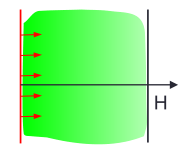
\includegraphics[width=2.5in]{images/dfs/plane-multiplying-geo.png}
  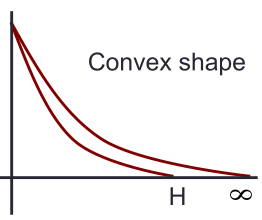
\includegraphics[width=2.5in]{images/dfs/plane-multiplying-phi.png}
  \caption{Plane Source in Finite Multiplying Medium with $\kinf < 1$}
\end{figure}
\end{enumerate}


\clearpage
\topic{Plane Source in Finite Multiplying Medium with $\kinf > 1$}
Consider a finite multiplying medium with $\kinf > 1$, it is a slab extending from $-H/2$ to $H/2$, it is subcritical with leakage, BC are from the current at center and the zero flux at the H/2 boundary. 
\eqn{ \dphidxn2 + B_m^2 \phi &= 0,  & B_m^2 &= \frac{\nu \Sigma_f - \Sigma_a}{D} = \frac{\kinf - 1}{L^2} > 0  &\phi(x) &= A \cos(B_mx) + B\sin(B_mx) }
BC1: $\phi(H/2) = 0$; BC2: $J(0) = \frac{S_0}{2}$. We can solve for the coefficients, and place absolute sign to represent the whole geometry: 
\eqn{ \phi(x) = \frac{S_0}{2DB_m \cos\left( \frac{B_m H}{2} \right)} \sin\left[ B_m \left(\frac{H}{2} - |x|\right) \right] }
Interpretations:
\begin{enumerate}
\item Because $\kinf > 1$, the flux shape is concave, that is, increasing negative slopes in the positive domain. In Fig.~\ref{approach-critical}, flux is convex when $\kinf < 1$ and concave when $\kinf > 1$, until we hit the cosine shape when $\keff = 1, \kinf = 1 + B^2L^2$ from 
  \eqn{ B^2 &= \frac{\frac{\nu \Sigma_f}{\keff} - \Sigma_a}{D} = \frac{\frac{\kinf}{\keff} - 1}{L^2}  & \kinf &= \keff + B^2 L^2}
\item If $H$ is increased to the critical dimension, that is, $H \to \frac{\pi}{B_m}$, then $\phi(0) \to \infty$; that is, if the reactor is critical, the flux at the source is infinite. That is, there is no steady-state solution for flux at the source site. In fact, if we place a fission detector at $x=0$ and measure source multiplication, 
  \eqn{M_s(0) = \frac{N_d \sigma_{f,d} V_d \phi(0)}{S_0} \propto \frac{\sigma_f}{2DB} \tan\left(\frac{BH}{2} \right) }
  Or the inverse source multiplication factor, 
  \eqn{ \frac{1}{M_s(0)} \propto \frac{1}{\tan\left(\frac{BH}{2} \right)} \to 0 }
\item To reach criticality, we can add fuel elements, withdraw control rods, and dilute boron. 1/M is useful for estimating criticality as shown in Figure~\ref{approach-critical}. 
  \begin{figure}[ht]
    \centering
    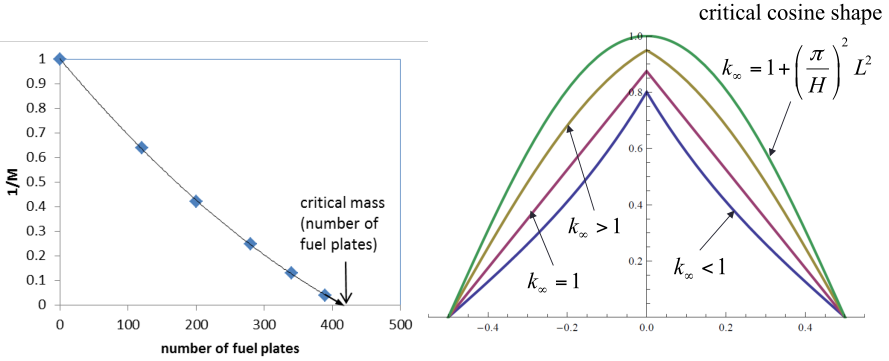
\includegraphics[width=5in]{images/dfs/approach-critical.png}
    \caption{1/M plot and Flux Shape In Approaching Criticality}\label{approach-critical}
  \end{figure}
\end{enumerate}




\clearpage
\topic{Summary}
\begin{enumerate}
\item \textbf{Super-positioning of sources}: if we are given a random source that is the sum of a couple of common forms of sources, we can super-position the flux from each of the common sources. This method works in any non-multiplying medium, and in multiplying medium in subcritical condition\footnote{Supercritical condition, as source increaes, flux inverts}. For instance, we can super-position point sources to get a line source. 

\item Diffusion theory is valid: 
  \begin{itemize}
    \item when there is little geometry heterogeneity;
    \item when $\Sigma_a \ll \Sigma_s$;
    \item when position is not too close to interface and source.
  \end{itemize}
  Diffusion theory is not valid near singularities. 

\item $\kinf$ is important\footnote{know this for the exams}: 
  \begin{itemize}
  \item $\kinf = 1$: flux is straight line;
  \item $\kinf < 1$ means $B^2 < 0$, flux is $\sinh, \cosh$ which is convex; 
  \item $\kinf > 1$ means $B^2 > 0$, flux is $\sin, \cos$ which is concave. 
  \end{itemize}
\end{enumerate}

  \begin{table}[ht]
    \centering
    \begin{tabular}{|c|c|c|c|c|} \hline
      Source & Geometry & Material &BCs & Flux \\ \hline \hline
      Point & $\infty$ Sphere & Non-multi.  & $\displaystyle \lim_{r\to\infty} \phi = 0, \lim_{r\to 0} 4 \pi r^2 J(r) = S_0$ & $\displaystyle \frac{S_0}{4\pi D} \frac{e^{-r/L}}{r}$ \\ \hline
      Plane & $\infty$ Slab & Non-multi. &$\displaystyle \lim_{x\to \infty} = 0, \lim_{x \to 0} J(x)  = \frac{S_0}{2}$ & $\displaystyle \frac{S_0 L}{2D} e^{-|x|/L}$ \\ \hline
      Plane & Finite Slab &Multi. $\kinf < 1$ & $\phi(0) = \phi_0, \phi(H) = 0$ & $\displaystyle \phi_0 \left[ \cosh(|B|x) - \coth(|B|H) \sinh(|B| x) \right]$ \\ \hline
      Plane & Finite Slab &Multi. $\kinf > 1$ & $\displaystyle \phi(H/2) = 0, J(0) = \frac{S_0}{2}$ & $\displaystyle \frac{S_0}{2D B_m \cos (BH/2)} \sin \left[ B \left( \frac{H}{2} - |x| \right) \right]$ \\ \hline
    \end{tabular}
    \caption{Subcritical System: Source and Flux} 
  \end{table}
  
  
\end{document}
